\chapter{\textbf{REVISÃO BIBLIOGRÁFICA}}
\section{\textbf{Acessibilidade no ensino superior e deficiência visual}}
 A inclusão de pessoas com deficiência no ensino superior é uma pauta cada vez mais presente na agenda de instituições acadêmicas, impulsionada tanto por legislações específicas quanto por demandas sociais urgentes. De acordo com IBGE, o Censo Demográfico de 2022 apontou que cerca de 3,6\% da população brasileira apresenta algum grau de deficiência visual severa, o que representa milhões de cidadãos potencialmente impactados por barreiras de acessibilidade física e informacional \cite{IBGE2023}.

 A garantia de acessibilidade nos espaços educacionais não deve ser entendida apenas como uma questão de infraestrutura, mas também como um direito fundamental assegurado pela Constituição Federal de 1988 e reforçado pelo Estatuto da Pessoa com Deficiência (Lei nº 13.146/2015). Esse marco legal estabelece que é dever do Estado, da sociedade e da família assegurar, com prioridade, a inclusão plena das pessoas com deficiência, o que inclui o acesso, a permanência e o sucesso no ensino superior. No entanto, a distância entre o previsto na legislação e a realidade cotidiana dos estudantes ainda é significativa, especialmente quando se trata de acessibilidade arquitetônica e informacional.

 Um levantamento nacional conduzido por \citeonline{Silva2020} aponta que estudantes com deficiência visual enfrentam maiores índices de evasão universitária, principalmente em cursos presenciais com ambientes físicos complexos. As dificuldades de locomoção autônoma e a dependência constante de terceiros para atividades simples, como se locomover entre prédios ou localizar salas, afetam diretamente sua autonomia e bem-estar psicológico.

 A UFMG, enquanto uma das maiores universidades federais do país, possui uma infraestrutura ampla e diversificada, com desafios evidentes para o deslocamento de pessoas com mobilidade reduzida ou deficiência sensorial. No campus Pampulha, a extensão territorial, a variação de terrenos e a sinalização insuficiente são aspectos frequentemente citados como obstáculos. Segundo \citeonline{Oliveira2019}, esses desafios estruturais impactam diretamente a experiência de alunos com deficiência, exigindo soluções complementares de acessibilidade. Nesse cenário, soluções tecnológicas específicas para esse contexto, como a proposta deste trabalho, podem atuar como complementos viáveis às políticas institucionais de inclusão, oferecendo suporte à autonomia de alunos com deficiência visual no cotidiano acadêmico.

 No contexto universitário, as barreiras assumem diversas formas, como a ausência de sinalização tátil, rotas acessíveis mal planejadas e a carência de tecnologias assistivas adequadas. Embora políticas de inclusão estejam presentes em muitas universidades brasileiras, como a Política Nacional de Educação Especial na Perspectiva da Educação Inclusiva \cite{Brasil2008}, a efetivação da acessibilidade plena nos campi ainda enfrenta entraves estruturais e orçamentários. A UFMG, por exemplo, possui iniciativas como o Núcleo de Acessibilidade e Inclusão, mas a extensão do campus da Pampulha e a diversidade de edificações e trajetos implicam desafios adicionais para a mobilidade autônoma de estudantes com deficiência visual \cite{Oliveira2019}.

 A mobilidade independente é um fator crítico para a permanência e o desempenho acadêmico desses estudantes. Tecnologias assistivas que proporcionem orientação espacial e reconhecimento de obstáculos em ambientes complexos, como o campus universitário, tornam-se, portanto, ferramentas de apoio essenciais. Estudos como os de \citeonline{Pereira2021} e \citeonline{Oliveira2019} evidenciam que o uso de recursos tecnológicos, desde bengalas eletrônicas até sistemas baseados em inteligência artificial, pode ampliar significativamente a autonomia e segurança dessas pessoas.
 
\section{\textbf{Tecnologias assistivas baseadas em visão computacional}}
As tecnologias assistivas são recursos, dispositivos, metodologias ou estratégias que têm como finalidade ampliar a funcionalidade de pessoas com deficiência, promovendo maior autonomia e inclusão. Segundo a definição da Associação Brasileira de Normas Técnicas (ABNT), tecnologias assistivas são produtos, equipamentos, dispositivos, recursos, metodologias, estratégias, práticas e serviços que objetivam proporcionar ou ampliar habilidades funcionais de pessoas com deficiência e, consequentemente, promover vida independente e inclusão \cite{ABNT2004}. No contexto da deficiência visual, essas tecnologias podem assumir formas como leitores de tela, bengalas eletrônicas, sistemas de localização auditiva e, mais recentemente, soluções baseadas em inteligência artificial. As Figuras \ref{fg-bengala}, \ref{fg-sinal} e \ref{fg-caneta} mostram algumas dessas tecnologias assistivas citadas anteriormente.
% --- INÍCIO Figura
\begin{figure}[htbp]
  \centering
  \caption{Bengala eletrônica}
  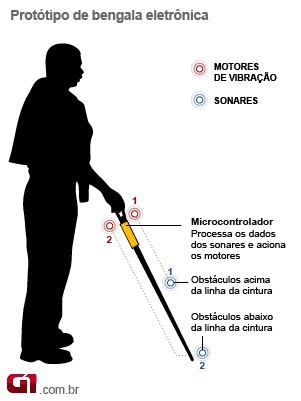
\includegraphics[width=0.4 \textwidth]{Figuras/bengala2.jpg}
  \\
  Disponível em: \url{https://www.deficienteciente.com.br/brasileiro-cria-bengala-eletronica-de-baixo-custo-para-deficientes-visuais.html} (Acessado em 01/04/2025)
  \label{fg-bengala}
\end{figure}
% --- FIM Figura

% --- Figura
\begin{figure}[htbp]
  \centering
  \caption{Sinalização por vibração}
  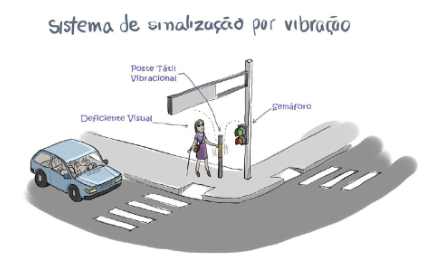
\includegraphics[width=0.6 \textwidth]{Figuras/sinal-vibra.png}
  \\
  Disponível em: \url{https://www.passeidireto.com/arquivo/79514730/deficiente-visual-e-o-transito-final} (Acessado em 01/04/2025)
  \label{fg-sinal}
\end{figure}
% --- Figura

% --- INÍCIO Figura
\begin{figure}[htbp]
  \centering
  \caption{Caneta falante}
  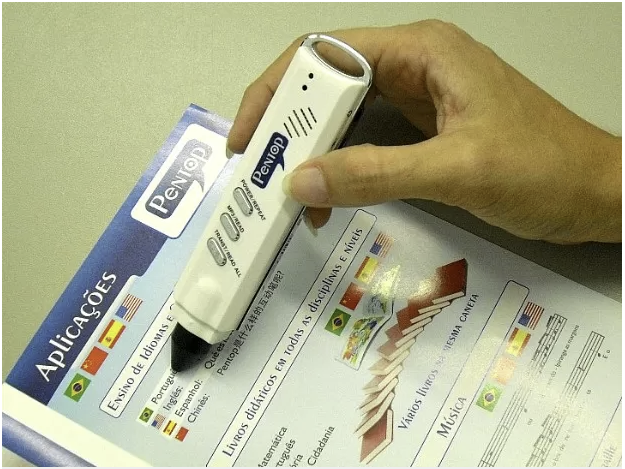
\includegraphics[width=0.8 \textwidth]{Figuras/caneta-fala.png}
  \\
  Disponível em: \url{https://g1.globo.com/am/amazonas/noticia/2012/09/caneta-que-fala-valor-do-dinheiro-para-deficientes-visuais-e-produzida-no-am.html} (Acessado em 01/04/2025)
  \label{fg-caneta}
\end{figure}
% --- FIM Figura

A visão computacional é um ramo da inteligência artificial que busca simular a capacidade humana de interpretar o ambiente por meio de imagens e vídeos. No campo da acessibilidade, ela tem sido empregada para desenvolver sistemas que reconhecem objetos, textos, rostos e sinais, oferecendo suporte para a orientação e interação de pessoas com deficiência visual com o mundo físico. Combinada a outros recursos, como sensores e \textit{feedback} auditivo, a visão computacional permite criar experiências assistivas mais ricas e contextualmente informadas \cite{Goodrich2020}.

Dentre as aplicações mais promissoras da visão computacional na assistência a pessoas cegas ou com baixa visão estão os sistemas de navegação autônoma em ambientes urbanos, o reconhecimento de sinais e placas, e a identificação de objetos em tempo real. Projetos como o Seeing AI, apresentado na Figura \ref{fg-seeing-ai}, da Microsoft, ou o OrCam MyEye, demonstram como dispositivos portáteis podem traduzir elementos visuais em áudio, promovendo independência funcional \cite{Li2021}. Embora esses sistemas tenham alcançado certo grau de sofisticação, ainda enfrentam limitações em ambientes muito específicos ou desorganizados, como é o caso de muitos campi universitários brasileiros.

% --- INÍCIO Figura
\begin{figure}[htbp]
  \centering
  \caption{Seeing Ai, Microsoft}
  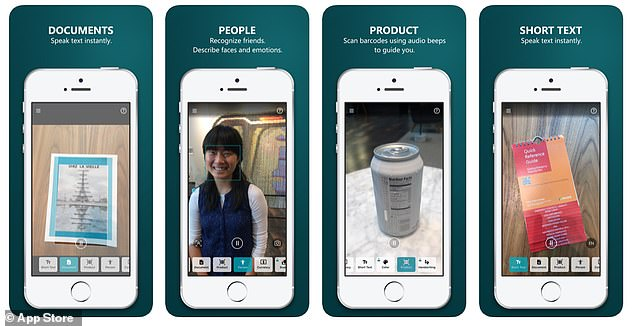
\includegraphics[width=0.8 \textwidth]{Figuras/seeing-ai.jpg}
  \\
  Disponível em: \url{https://ixd.prattsi.org/2024/09/assistive-technology-microsoft-seeing-ai/} (Acessado em 01/04/2025)
  \label{fg-seeing-ai}
\end{figure}
% --- FIM Figura

Apesar dos avanços, a maior parte dos sistemas comerciais apresenta limitações de contexto e adaptabilidade. Estudos como o de \citeonline{Martins2022} indicam que soluções importadas muitas vezes não se ajustam à realidade arquitetônica e cultural brasileira, seja por dificuldades na segmentação semântica de ambientes abertos, seja por falhas na detecção de objetos urbanos comuns no Brasil, como pontos de ônibus não padronizados ou faixas de pedestres pouco visíveis. Isso reforça a importância do desenvolvimento de sistemas contextualmente situados, com bases de dados e treinos locais, como proposto neste trabalho.

Uma característica central das tecnologias assistivas baseadas em visão computacional é o modo como os dados visuais são traduzidos em informação acessível. O \textit{feedback} auditivo é uma das interfaces mais eficazes para usuários com deficiência visual, pois permite a interpretação imediata de informações ambientais sem a necessidade de leitura tátil ou intervenção manual. Segundo \citeonline{Nguyen2020-feedback_strategies}, o uso de sinais auditivos diretos e contextuais reduz o tempo de resposta do usuário e aumenta sua percepção de controle sobre o ambiente, especialmente quando integrado com reconhecimento de objetos em vídeo.

Portanto, a aplicação da visão computacional com suporte de inteligência artificial em contextos assistivos não só é viável, como desejável do ponto de vista técnico e social. O uso de algoritmos robustos como o YOLO versão 11 (YOLOv11), que oferecem detecção em alta velocidade e com alta precisão, representa um avanço relevante frente aos métodos mais tradicionais. Como apontam \citeonline{redmon2018}, modelos da família YOLO são especialmente indicados para aplicações em tempo real e ambientes não controlados, características que se alinham perfeitamente à proposta deste trabalho no campus universitário.

\section{\textbf{Detecção de Objetos com Inteligência Artificial: O Algoritmo YOLOv11}}

Neste capítulo, são apresentados os fundamentos técnicos que sustentam o desenvolvimento da ferramenta proposta neste trabalho, com ênfase em visão computacional, aprendizado profundo e detecção de objetos com o algoritmo YOLOv11.

\subsection{\textbf{Fundamentos de Visão Computacional e Aprendizado Profundo}}

A visão computacional é um campo interdisciplinar que visa permitir que computadores interpretem e compreendam imagens e vídeos, simulando a capacidade perceptiva dos seres humanos, como mostrado na Figura \ref{fg-visao-computacional}. Essa área envolve diversas etapas, como a aquisição de imagens, o processamento digital, a análise e a interpretação de informações visuais. Ao longo das últimas décadas, avanços significativos em algoritmos, aumento de poder computacional e disponibilidade de grandes volumes de dados tornaram essa disciplina uma base essencial para soluções modernas em inteligência artificial  \cite{szeliski2022}.

% --- INÍCIO Figura
\begin{figure}[htbp]
  \centering
  \caption{Visão computacional - similaridade com percepção humana}
  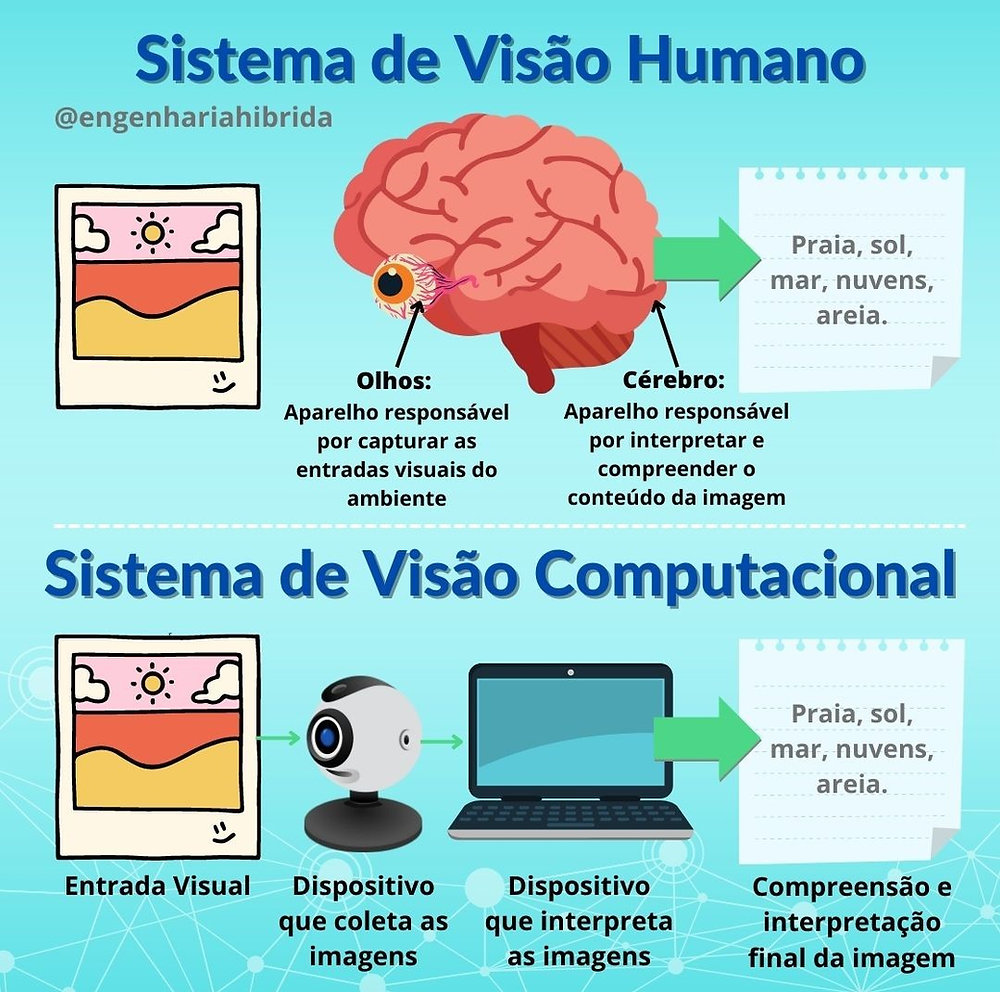
\includegraphics[width=0.8 \textwidth]{Figuras/visao-computacional.jpg}
  \\
  Disponível em: \url{https://www.engenhariahibrida.com.br/post/visao-computacional-como-funciona} (Acessado em 01/04/2025)
  \label{fg-visao-computacional}
\end{figure}
% --- FIM Figura

A aplicação da visão computacional se estende a diversas áreas, como medicina (diagnóstico por imagem), indústria (inspeção de qualidade), segurança (reconhecimento facial), transportes (veículos autônomos) e, mais recentemente, acessibilidade. Em contextos assistivos, sua aplicação visa melhorar a interação de pessoas com deficiência visual com o ambiente, oferecendo soluções de detecção e descrição auditiva de objetos e espaços \cite{goodfellow2016}.

A transformação mais significativa da visão computacional ocorreu com a introdução do aprendizado profundo, especialmente com as redes neurais convolucionais (CNNs). Essas redes se tornaram fundamentais para a análise de dados visuais, pois conseguem extrair características complexas das imagens de forma autônoma, sem necessidade de engenharia manual de atributos \cite{gu2018}.

Com a disseminação de ferramentas como TensorFlow, Keras e PyTorch, o desenvolvimento de aplicações de visão computacional com aprendizado profundo foi amplamente democratizado. Essas bibliotecas de utilização livre (\textit{open source}) permitem que pesquisadores e desenvolvedores criem modelos personalizados com maior facilidade, acelerando o processo de prototipagem e implantação \cite{hassaballah2020}.

Por fim, o avanço do \textit{hardware}, especialmente unidades de processamento gráfico (GPUs) e as unidades de processamento de tensor (TPUs), e a popularização de dispositivos móveis com capacidade de processamento elevado ampliaram ainda mais o campo de aplicação da visão computacional. Atualmente, sistemas inteligentes com reconhecimento de imagem podem ser executados em \textit{smartphones}, possibilitando aplicações portáteis e acessíveis, como é o caso do presente trabalho voltado para usuários com deficiência visual \cite{geron2022}.

\subsection{\textbf{Conceitos Básicos de Aprendizado Profundo}}

O aprendizado profundo é uma subárea do aprendizado de máquina que utiliza redes neurais artificiais com várias camadas para aprender representações hierárquicas dos dados. Essas redes são capazes de identificar padrões complexos por meio de sucessivas transformações não lineares dos dados de entrada, aproximando-se do comportamento de redes neurais biológicas \cite{goodfellow2016}).

Um dos principais diferenciais do aprendizado profundo é a sua capacidade de realizar a extração automática de características. Isso significa que, ao contrário de técnicas mais tradicionais, não há necessidade de que especialistas definam previamente os atributos que serão analisados: a própria rede aprende essas representações a partir dos dados \cite{Agarwal2021-deeplearning}.

A estrutura dessas redes, mostrada na Figura \ref{fg0}, inclui uma camada de entrada, múltiplas camadas ocultas e uma camada de saída. Cada camada realiza cálculos com base nas saídas das camadas anteriores, e as conexões entre os neurônios são ponderadas por valores ajustáveis durante o treinamento. Funções de ativação como a unidade linear retificada (ReLU) são essenciais para introduzir não linearidades no modelo, permitindo a representação de relações complexas \cite{gu2018}.

% --- Figura
\begin{figure}[htbp]
  \centering
  \caption{Estrutura de uma rede neural profunda}
  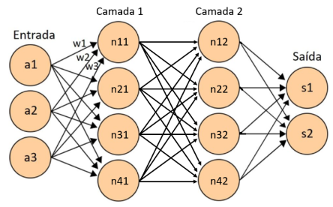
\includegraphics[width=0.6\textwidth]{Figuras/Est-rede-neural-profunda.png}
  \\
  Disponível em: \url{https://didatica.tech/introducao-a-redes-neurais-e-deep-learning/} (Acessado em 01/04/2025)
  \label{fg0}
\end{figure}
% --- Figura

\subsection{\textbf{Redes Neurais Convolucionais para Reconhecimento de Objetos}}
As CNNs foram projetadas especificamente para lidar com imagens. Inspiradas na organização do córtex visual dos mamíferos, essas redes exploram relações espaciais locais por meio do uso de filtros convolucionais, que varrem a imagem identificando padrões específicos em diferentes regiões \cite{lecun2015}.

Uma CNN, como mostrado na Figura \ref{fg-cnn}, é composta por várias camadas: convolucionais, de \textit{pooling} e totalmente conectadas. As camadas convolucionais aplicam filtros que produzem mapas de ativação, nos quais são realçadas características como bordas ou formas. As camadas de \textit{pooling} têm a função de reduzir a resolução espacial desses mapas, diminuindo a complexidade computacional e ajudando a evitar o sobreajuste \cite{gu2018}.

% --- Figura
\begin{figure}[htbp]
  \centering
  \caption{Estrutura de uma rede neural profunda}
  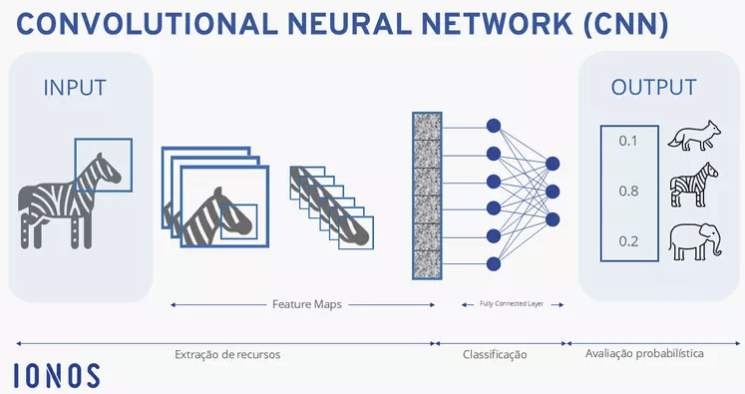
\includegraphics[width=0.8\textwidth]{Figuras/cnn.png}
  \\
  Disponível em: \url{https://www.ionos.com/pt-br/digitalguide/sites-de-internet/desenvolvimento-web/convolutional-neural-network/} (Acessado em 01/04/2025)
  \label{fg-cnn}
\end{figure}
% --- Figura

Um marco importante foi a criação da AlexNet em 2012, que venceu a competição ImageNet, demonstrando o potencial das CNNs em tarefas de larga escala \cite{krizhevsky2012}. Desde então, arquiteturas como VGG, GoogLeNet e ResNet ampliaram a profundidade e a eficiência das redes, contribuindo para a evolução da detecção de objetos.

A Figura \ref{fg1} detalha a arquitetura de AlexNet, uma rede neural convolucional que revolucionou a visão computacional ao vencer a competição ImageNet em 2012.

% --- Figura
\begin{figure}[htbp]
  \centering
  \caption{Arquitetura do AlexNet}
  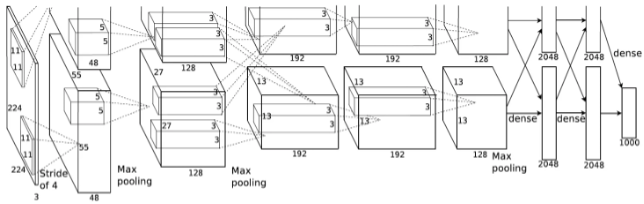
\includegraphics[width=1.0\textwidth]{Figuras/arquitetura-alexnet.png}
  \\
  Disponível em: \url{https://jefferson023.medium.com/alexnet-para-classifica%C3%A7%C3%A3o-de-imagens-d86c482a44b3} \\(Acessado em 01/04/2025)
  \label{fg1}
\end{figure}
% --- Figura

A eficiência computacional das CNNs permite que esses modelos sejam aplicados em tempo real ou quase tempo real, o que é essencial para sistemas assistivos com resposta imediata ao usuário \cite{bochkovskiy2020}.

\subsection{\textbf{Evolução e Funcionamento do Algoritmo YOLO}}

O algoritmo YOLO revolucionou a detecção de objetos ao propor uma abordagem unificada e extremamente rápida. Em vez de seguir o paradigma tradicional, que separava a tarefa em etapas como geração de propostas de região e posterior classificação, o YOLO trata toda a detecção como um problema de regressão direta, em que uma única rede neural realiza todas as previsões simultaneamente \cite{redmon2016}.

A imagem de entrada é dividida em uma grade, e cada célula dessa grade é responsável por prever várias caixas delimitadoras e suas respectivas probabilidades de classe. Essa abordagem permite que a detecção seja extremamente rápida, o que é essencial para aplicações em tempo real \cite{bochkovskiy2020}.

Como ilustrado na Figura \ref{fg2}, o algoritmo YOLO é capaz de realizar a detecção de objetos em tempo real, identificando múltiplos objetos em uma única imagem e delineando-os com \textit{bounding boxes}.

% --- Figura
\begin{figure}[htbp]
  \centering
  \caption{Detecção de objetos em tempo real com o YOLO}
  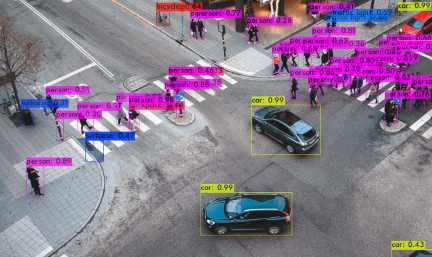
\includegraphics[width=1\textwidth]{Figuras/detec-yolo.png}
  \\
  Disponível em: \url{https://iaexpert.academy/2020/10/13/deteccao-de-objetos-com-yolo-uma-abordagem-moderna/?doing_wp_cron=1719375630.4834909439086914062500 } \\(Acessado em 01/04/2025)
  \label{fg2}
\end{figure}
% --- Figura

As versões subsequentes do YOLO, v3, v4, v5 até a v12, introduziram diversas melhorias, incluindo redes mais profundas, camadas residuais, normalização por lotes e previsão em múltiplas escalas \cite{bochkovskiy2020}.

O YOLOv11, desenvolvido pela Ultralytics, conta com uma infraestrutura moderna baseada em PyTorch, suporte nativo a exportação para ONNX e TensorRT, e integração com vídeos em tempo real, o que o torna altamente eficiente para aplicações práticas \cite{Ultralytics2024}.

\subsection{\textbf{Aplicação do YOLO em Tecnologias Assistivas}}

A detecção de objetos com o algoritmo tem sido amplamente explorada em projetos de tecnologias assistivas voltadas para pessoas com deficiência visual. A capacidade do algoritmo de realizar detecções em tempo real com alta precisão o torna ideal para aplicações que exigem respostas imediatas, como é o caso de sistemas de orientação pessoal e navegação urbana \cite{redmon2016}.

Diversos estudos têm utilizado o YOLO para construir sistemas portáteis que auxiliam deficientes visuais a identificar objetos e interagir com o ambiente. Por exemplo, \citeonline{Nguyen2020-smart_glasses} desenvolveram um sistema baseado em YOLOv3 embarcado em óculos inteligentes que detecta sinais de trânsito e envia mensagens de voz ao usuário. Outros projetos, como o de \citeonline{Khan2021}, usaram o YOLOv4 para detectar degraus, portas e semáforos, auxiliando na mobilidade autônoma em espaços urbanos.

A robustez do YOLO para detectar objetos diversos em diferentes condições ambientais é uma de suas principais vantagens em cenários assistivos. Isso permite que o algoritmo seja aplicado em ambientes dinâmicos e pouco padronizados, como é o caso de ruas, praças e campi universitários. Além disso, sua compatibilidade com dispositivos embarcados facilita a construção de sistemas de baixo custo e alta portabilidade \cite{bochkovskiy2020}.

Apesar de suas qualidades, o uso do YOLO em aplicações assistivas também enfrenta desafios. Entre eles estão a detecção de objetos pequenos ou parcialmente ocultos e a variabilidade de iluminação nos ambientes reais. Estudos como o de \citeonline{Li2022} apontam que a acurácia do algoritmo pode ser comprometida em condições adversas, o que reforça a necessidade de adaptações e treinamento com dados contextualizados.

\section{\textbf{Construção de conjunto de dados personalizados}}

A construção de conjunto de dados (\textit{datasets}) personalizados é uma etapa fundamental no desenvolvimento de sistemas de visão computacional baseados em aprendizado profundo. Enquanto grandes bancos de dados públicos, como ImageNet, COCO e Open Images, são amplamente utilizados para treinamentos genéricos, aplicações específicas exigem conjuntos de dados adaptados ao contexto e aos objetivos do projeto \cite{Zhou2017}.

Em projetos voltados para acessibilidade, como sistemas de assistência para pessoas com deficiência visual, a construção de um \textit{dataset} personalizado permite que o modelo aprenda padrões visuais diretamente relacionados ao ambiente de uso. Isso é particularmente importante em ambientes urbanos ou universitários, nos quais a variação de elementos arquitetônicos, sinalização e objetos é significativa e muitas vezes fora do escopo dos \textit{datasets} públicos \cite{Khan2021}.

A construção de um \textit{dataset} personalizado segue algumas etapas essenciais: i. captura de imagens ou vídeos, ii. seleção e extração de \textit{frames}, iii. anotação das \textit{bounding boxes} e, iv. classificação dos objetos. Diversas ferramentas auxiliam nesse processo, como o LabelImg, VoTT e o Roboflow, que oferecem interfaces intuitivas para rotulagem e exportação em formatos compatíveis com os principais modelos de detecção \cite{Tzutalin2015}.

Outro aspecto crítico é a qualidade e diversidade dos dados. Para que um modelo generalize bem, o \textit{dataset} deve incluir variações de iluminação, perspectiva, escala e posicionamento dos objetos. Técnicas de \textit{data augmentation}, como rotação, inversão, ajuste de brilho e aplicação de ruído, são comumente empregadas para ampliar artificialmente o volume de exemplos sem comprometer a veracidade das informações \cite{Shorten2019}.

Por fim, é importante que o \textit{dataset} reflita não apenas a variedade de situações do mundo real, mas também os objetivos da aplicação. Em projetos assistivos, por exemplo, pode ser mais relevante rotular elementos como rampas, escadas, sinalização auditiva ou superfícies táteis, em vez de objetos comuns como carros ou pessoas. A adequação do \textit{dataset} ao contexto real de uso é o que garante a efetividade prática do modelo treinado.

\section{\textbf{Sinais Auditivos e \textit{Feedback} em Sistemas Assistivos}}

Os sinais auditivos são amplamente utilizados como mecanismo de \textit{feedback} em tecnologias assistivas voltadas para pessoas com deficiência visual. Por meio de sons, alertas ou mensagens de áudio, esses sistemas fornecem informações essenciais sobre o ambiente, promovendo maior autonomia e segurança aos usuários \cite{Milella2014}.

A principal vantagem do \textit{feedback} auditivo é a capacidade de transmitir informações de forma não visual, liberando o sentido da audição para suprir a falta de percepção visual. Estudos mostram que sinais auditivos bem projetados contribuem significativamente para a localização de objetos, orientação espacial e prevenção de acidentes \cite{Nguyen2020-feedback_strategies}.

Existem diferentes abordagens para a implementação de \textit{feedback} auditivo em sistemas assistivos. Algumas utilizam sons padronizados para indicar a presença de um objeto, enquanto outras se valem de mensagens de voz geradas dinamicamente. A escolha da abordagem depende do tipo de informação a ser transmitida, da urgência do alerta e do contexto de uso \cite{Spagnol2018}.

Um desafio importante é evitar a sobrecarga auditiva do usuário. Sistemas que emitem muitos sons ou mensagens em sequência podem causar distração ou confusão. Por isso, boas práticas envolvem a hierarquização dos alertas, uso de sons distintos e ajustes dinâmicos de volume com base no nível de ruído ambiente \cite{Akbar2022}.

Diversos dispositivos já exploram com sucesso o uso de \textit{feedback} auditivo, como o OrCam MyEye - mostrado na Figura \ref{fg-orcammyeye}, o projeto Microsoft Seeing AI e soluções embarcadas com Raspberry Pi. Esses exemplos demonstram a viabilidade e a eficácia do uso de sinais auditivos como ponte entre a interpretação visual automatizada e a comunicação com o usuário final.

% --- Figura
\begin{figure}[htbp]
  \centering
  \caption{OrCam MyEye}
  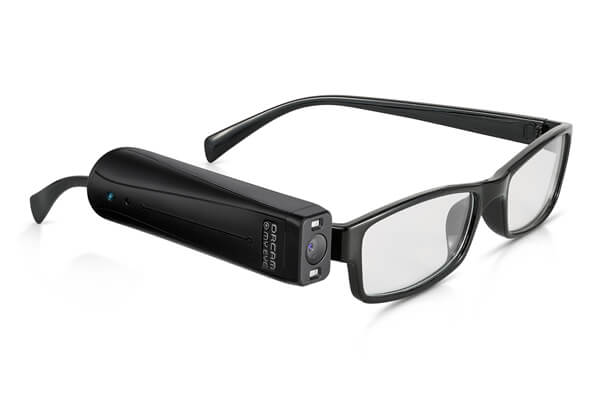
\includegraphics[width=0.8\textwidth]{Figuras/orcammyeye.jpg}
  \\
  Disponível em: \url{https://maisautonomia.com.br/produto/orcam-myeye-2-0/} \\(Acessado em 01/04/2025)
  \label{fg-orcammyeye}
\end{figure}
% --- Figura

\section{\textbf{Dispositivos e Plataformas para Tecnologias Assistivas Visuais}}

O desenvolvimento de dispositivos e plataformas tecnológicas voltados para pessoas com deficiência visual tem se expandido significativamente nos últimos anos, impulsionado pelos avanços em inteligência artificial, miniaturização de componentes e acessibilidade digital. Esses sistemas visam fornecer informações contextuais sobre o ambiente por meio de canais alternativos à visão, como a audição ou o tato, promovendo maior autonomia e inclusão \cite{Saeedi2021}.

Entre os dispositivos mais comuns estão os vestíveis do dia a dia, como óculos inteligentes e pulseiras sensoriais, que capturam dados do ambiente por meio de câmeras, sensores ultrassônicos, LiDAR e GPS, assim como fornecem \textit{feedback} em tempo real. Uma das iniciativas mais conhecidas é o OrCam MyEye, um pequeno dispositivo acoplado a óculos comuns, capaz de ler textos, reconhecer rostos e objetos, emitindo mensagens auditivas para o usuário \cite{OrCam2022}.

Outra plataforma amplamente reconhecida é o Microsoft Seeing AI, um aplicativo gratuito para \textit{smartphones} que utiliza visão computacional para descrever cenas, identificar produtos, reconhecer textos e até emoções faciais. O Seeing AI é um exemplo de solução acessível e eficaz, pois utiliza o \textit{hardware} já disponível em celulares modernos, dispensando a aquisição de dispositivos específicos \cite{Microsoft2023}.

Outras soluções têm apostado na integração de sensores múltiplos para oferecer navegação segura em tempo real. O projeto BLAID da Toyota, por exemplo, propõe um dispositivo vestível que combina visão computacional com sensores de profundidade para detectar obstáculos e orientar o deslocamento em ambientes internos, como corredores e escadas \cite{Toyota2018}.

Além dos dispositivos vestíveis e aplicativos móveis, plataformas embarcadas como Raspberry Pi e Arduino são comumente utilizadas em projetos de pesquisa e prototipagem rápida. Essas placas de baixo custo permitem a criação de sistemas personalizados, com câmeras e atuadores auditivos, sendo muito utilizadas em ambientes acadêmicos como parte de soluções educacionais acessíveis \cite{Pino2020}.

A escolha entre dispositivos dedicados e soluções baseadas em \textit{smartphones} depende de fatores como custo, portabilidade, facilidade de uso e escalabilidade. Aplicativos móveis são vantajosos pela ubiquidade dos celulares e atualização constante via \textit{software}, enquanto dispositivos dedicados, como óculos inteligentes, oferecem maior integração sensorial e desempenho específico \cite{Saeedi2021}.

Por fim, é importante destacar que a eficácia desses dispositivos não depende apenas de sua sofisticação tecnológica, mas também da sua usabilidade e adaptação ao contexto do usuário. Sistemas com interfaces intuitivas, comandos por voz e \textit{feedback} personalizado são os que tendem a gerar maior aceitação e impacto positivo na vida de pessoas com deficiência visual. A revisão das plataformas existentes contribui, portanto, para fundamentar as escolhas tecnológicas feitas no presente trabalho.

\section{\textbf{Avaliação da Efetividade em Tecnologias Assistivas}}
A avaliação da efetividade de tecnologias assistivas é uma etapa essencial para garantir que as soluções tecnológicas desenvolvidas realmente atendam às necessidades dos usuários com deficiência. Esse processo vai além da validação técnica e contempla aspectos como usabilidade, acessibilidade, satisfação do usuário, segurança e impacto na qualidade de vida \cite{Wentz2013}.

Um dos principais métodos para avaliação de sistemas assistivos é a aplicação de testes com usuários reais em ambientes controlados e em situações reais de uso. Esses testes permitem identificar barreiras de uso, falhas de comunicação entre sistema e usuário, e oportunidades de melhoria. O uso de entrevistas, questionários e observação direta são ferramentas valiosas nesse contexto \cite{Kintsch2002}.

Outra abordagem relevante é a aplicação de instrumentos padronizados de avaliação, como a escala de usabilidade do sistema, que fornece um índice quantitativo da usabilidade percebida pelo usuário. Esses instrumentos têm a vantagem de permitir a comparação entre diferentes tecnologias e protótipos, oferecendo uma base objetiva para tomada de decisão sobre aprimoramentos \cite{Brooke1996}.

A avaliação também deve considerar os princípios das diretrizes internacionais de acessibilidade digital mesmo quando o sistema não for estritamente digital. Esses princípios ajudam a garantir que as interfaces, alertas auditivos e formas de interação sejam compatíveis com diferentes perfis de usuários \cite{W3C2023}.

Estudos de caso com aplicação em campo são considerados uma das formas mais ricas de avaliação, pois permitem observar o impacto da tecnologia em situações reais e sob condições não controladas. Avaliações longitudinais, com acompanhamento ao longo do tempo, são especialmente valiosas para verificar adesão ao uso e impactos duradouros \cite{Batavia1990}.

Por fim, o envolvimento direto dos usuários com deficiência visual em todas as fases do desenvolvimento e da avaliação do sistema contribui para a construção de soluções centradas nas pessoas. Essa abordagem participativa tem sido promovida como uma boa prática no âmbito do design universal e da inclusão digital \cite{Story1998}.

\section{\textbf{Ética e Responsabilidade no Uso de Inteligência Artificial Assistiva}}

O uso de inteligência artificial (IA) em tecnologias assistivas levanta questões éticas relevantes que vão além da eficiência técnica. Ao lidar com dados sensíveis, como imagens do ambiente e comportamentos dos usuários, esses sistemas devem ser projetados considerando princípios como privacidade, segurança, transparência e não discriminação \cite{Floridi2018}.

A coleta e o processamento de imagens em tempo real, por exemplo, podem expor terceiros inadvertidamente, levantando preocupações sobre consentimento e anonimato. Em ambientes universitários ou urbanos, onde há tráfego constante de pessoas, é fundamental garantir que os dados captados não sejam armazenados indevidamente ou utilizados para outros fins sem autorização \cite{Jobin2019}.

Outro aspecto crítico é o viés algorítmico. Modelos de IA treinados com bases de dados pouco diversificadas podem apresentar desempenho inferior para determinados grupos, perpetuando desigualdades. Em tecnologias assistivas, isso pode significar falhas na detecção de objetos relevantes em contextos específicos, como escolas públicas, periferias ou comunidades rurais \cite{Buolamwini2018}.

A transparência também é uma exigência crescente. Usuários de sistemas assistivos têm direito a compreender como as decisões são tomadas, como os dados são processados e que garantias existem contra erros. Para isso, boas práticas incluem o fornecimento de informações acessíveis, documentação clara e possibilidade de auditoria \cite{Morley2020}.

Responsabilidade legal também é um ponto sensível: quem responde por falhas de um sistema assistivo automatizado? Fabricante, desenvolvedor, instituição usuária? A ausência de regulamentações específicas para IA em muitos países torna essencial a adoção de princípios de ética por design, ou seja, a incorporação de valores humanos e sociais desde o início do desenvolvimento \cite{Dignum2019}.

Esforços internacionais como o da Organização das Nações Unidas para a Educação, a Ciência e a Cultura (UNESCO) e da União Europeia têm buscado estabelecer diretrizes para o uso ético da IA. O Brasil também avança com a Estratégia Brasileira de Inteligência Artificial, que destaca a inclusão, a proteção de dados e os direitos humanos como pilares para o uso consciente dessas tecnologias \cite{MCTI2021}.

\section{\textbf{Considerações Finais}}

Diante desse cenário, este trabalho busca contribuir com a inclusão universitária por meio do desenvolvimento de uma ferramenta baseada em visão computacional, capaz de reconhecer elementos do ambiente físico da UFMG e fornecer \textit{feedback} auditivo em tempo real ao usuário com deficiência visual. A seguir, discute-se o panorama das tecnologias assistivas baseadas em visão computacional. 

Para que sistemas assistivos baseados em visão computacional sejam eficazes, é essencial que estejam sintonizados com o ambiente onde serão utilizados. A utilização de vídeos capturados diretamente no campus da UFMG e a construção de um \textit{dataset} com objetos de interesse locais, como faixas de pedestre, bancos e placas, permite uma adaptação do sistema às condições reais de uso. Essa abordagem é consistente com recomendações de estudos recentes, que destacam a importância da coleta de dados em contextos específicos para aumentar a precisão da detecção e a usabilidade final \cite{Borges2023}. 